\documentclass[11pt]{article}
\usepackage[letterpaper]{geometry}
\usepackage{MATH561}

\begin{document}
\noindent \textbf{\Large{Caleb Logemann \\
MATH 561 Numerical Analysis I \\
Homework 2
}}

\begin{enumerate}
    \item
        \begin{enumerate}
            \item[(a)] \hfill \\
                \begin{center}
                    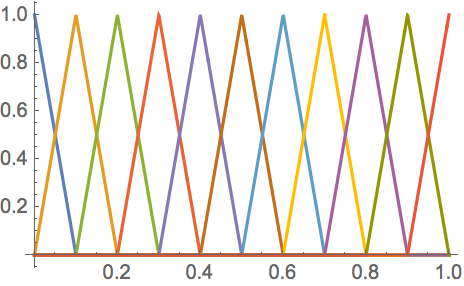
\includegraphics[scale=.5]{Figures/02_1a.png}
                \end{center}

            \item[(b)]
                If $j = k$, then $\pi_j\p{k/n} = \pi_j{j/n} = 1$.
                If $j \neq k$, then $\pi_j\p{k/n} = 0$, because $k/n$ is
                outside of the division that is the support of $\pi_j$

            \item[(c)]
                Let $c_0, c_1, \ldots, c_n \in \RR$ be given such that
                $\sum{i=0}{n}{c_i \pi_i\p{t}} = 0$ for all $t \in \p{0,1}$
                Consider $t = k/n$ for some $k \in \set{0, 1, \ldots, n}$, then
                $\sum{i=0}{n}{c_i \pi_i\p{k/n}} = c_k \pi_k\p{k/n}$, because
                $\pi_j{k/n} = 0$ for all $j \neq k$.
                Also $\pi_k\p{k/n} = 1$, so $c_k \pi_k\p{k/n} = c_k$.
                However this sum must be equal to $0$ at $t = k/n$, so $c_k = 0$.
                This implies that $c_0 = c_1 = \cdots = c_n = 0$.
                Thus the $\set{\pi_j}_{j=0}^n$ is linearly independent over the
                interval $(0, 1)$.
                This also implies that $\set{\pi_j}_{j=0}^n$ is linearly independent 
                over the points $\set{0, 1/n, \ldots, \frac{n-1}{n}, 1}$, because
                at these points only one of the functions contributes to the
                overall sum.

            \item[(d)]
                
        \end{enumerate}
    \item % #2 finding upper bounds for error
        \begin{enumerate}
            \item[(a)]
                
            \item[(b)]
        \end{enumerate}
    \item
    \item
    \item
    \item % #6
        \begin{enumerate}
            \item[(a)]

            \item[(b)]
                \begin{enumerate}
                    \item[(b.1)]
                    \item[(b.2)]
                    \item[(b.3)]
                \end{enumerate}
        \end{enumerate}
    \item
    \item
\end{enumerate}
\end{document}
